\documentclass[lettersize,journal]{IEEEtran}
\usepackage{amsmath,amsfonts}
\usepackage{algorithmic}
\usepackage{algorithm}
\usepackage{array}
\usepackage[caption=false,font=normalsize,labelfont=sf,textfont=sf]{subfig}
\usepackage{textcomp}
\usepackage{stfloats}
\usepackage{url}
\usepackage{verbatim}
\usepackage{graphicx}
\usepackage{cite}
\usepackage{tikz}
\usetikzlibrary{positioning, calc, shapes, arrows, fit}
\usepackage{circuitikz}
\hyphenation{op-tical net-works semi-conduc-tor IEEE-Xplore}
\graphicspath{{images/}}
% updated with editorial comments 8/9/2021

\begin{document}

\title{Lab 1 -- Measuring ``Parasitic'' Properties\\of Passive Components with a VNA}

\author{Benjamin Sage\\Lab Partners: Marc Huerta, Devorah Simon}

% The paper headers
\markboth{EE 133: Analog Communications Design Laboratory, February~2022}%
{Shell \MakeLowercase{\textit{et al.}}: A Sample Article Using IEEEtran.cls for IEEE Journals}

% \IEEEpubid{0000--0000/00\$00.00~\copyright~2021 IEEE}
% Remember, if you use this you must call \IEEEpubidadjcol in the second
% column for its text to clear the IEEEpubid mark.

\maketitle

\begin{abstract}

Two passive components (capacitors and inductors) are analyzed using a Vector Network Analyzer (VNA) to see where they deviate from their theoretical behavior. This analysis gives rise to an important discovery known as self-resonant frequency. 
\end{abstract}

% \begin{IEEEkeywords}
% Article submission, IEEE, IEEEtran, journal, \LaTeX, paper, template, typesetting.
% \end{IEEEkeywords}

\section{Introduction}
\IEEEPARstart{I}{n} real life, electronic components deviate from their theoretical models:

\begin{align}
Z_R &= R \\
Z_C &= \frac{1}{j \omega C} = -\frac{j}{\omega C} \\
Z_L &= j \omega L
\end{align}

This is because, even though internally all components obey Maxwell's equations, manufactured {\bf{resistors}}, {\bf{capacitors}}, and {\bf{inductors}} are lumped combinations of simple mathematical models. Each of the three components---in real life---actually must be modeled using each of the three mathematical models. The amount that these components deviate depends on the frequency of the signal. For this reason, they can be analyzed using a Vector Network Analyzer (VNA).

After taking our measurements, we can compare our results to theoretical models using LTSpice.

\section{Experimental Setup}

\begin{figure*}[!t]
\centering
\subfloat[]{\includegraphics[width=2.5in]{vna}%
\label{fig_first_case}}
\hfil
\subfloat[]{\includegraphics[width=2.5in]{nwdz}%
\label{fig_second_case}}
\caption{The primary tools used in the experiemnt. (a) NanoVNA. (b) RF Demo Kit.}
\label{fig_sim}
\end{figure*}

Each of the electronic components analyzed are mounted to the RF Demo Kit ({\it{NWDZ Rev-01-10}}) seen in Fig. 1(a). Analysis was conducted using the NanoVNA in Fig. 1(b).

\section{Measurements and Results}

\subsection{Capacitor}

\begin{table}
\renewcommand{\arraystretch}{2.2}
\begin{center}
\caption{Measured Log Data of Capacitor.}
\label{tab1}
\begin{tabular}{c c c}
\hline
\bfseries Frequency (MHz) & $\mathbf{|S_{11}|}$ & $\mathbf{|S_{21}|}$\\
\hline
1.0 & 0 & -17\\
\hline
34.0 & -18 & -1\\ 
\hline
67.0 & -23 & 0\\
\hline 
100.0& -15 & 0\\
\hline
\end{tabular}
\end{center}
\end{table}

To identify the self-resonant frequency of the capacitor, we varied the frequencies from $1 \, \text{MHz}$ to $100 \, \text{MHz}$ and measured the S-Parameters $S_{11}$ and $S_{21}$ at each value. The results are depicted in {\bf{Table 1}}. A graph visualizing the relationship can be seen in Fig. 2.

We can see that the magnitude of $S_{11}$ dips as the frequency increases, up to a point. Around $50 \, \text{MHz}$, the plot reaches a minimum and begins to increase again.

The same effect is visible on the smith chart found in Fig. 3. Here, we see that the capacitor begins conductive, but as the frequency increases, it actually begins to act like an inductor. The crossover point here is clearly seen to be $51.51 \, \text{MHz}$. Thus, we have our self-resonant frequency:

\begin{equation}
\text{SRF}_C = 51.51 \, \text{MHz}
\end{equation}

\begin{figure}[!t]
\centering
\includegraphics[width=2.5in]{capacitor-smith}
\caption{Smith Chart Plot for Capacitor}
\label{fig_1}
\end{figure}

\begin{figure}[!t]
\centering
\includegraphics[width=2.5in]{capacitor-log}
\caption{Log Plot for Capacitor}
\label{fig_1}
\end{figure}


\subsection{Inductor}

For the inductor, we performed a similar frequency variation using the VNA. We measured the S-Parameters $S_{11}$ and $S_{21}$ for the inductor, varying the frequency from 100 MHz to 1,000 MHz.

Results were similar to the capacitor, but in the opposite direction. As expected, at low frequencies the inductor began by acting inductive, but at higher frequencies, it crossed into the lower (capacitive) side of the Smith Chart. These results are seen in Fig. 4.

Close analysis of the Smith Chart reveals the exact place the inductor crossed over: $393.88 \, \text{MHz}$. This gives us the important result:

\begin{equation}
\text{SRF}_L = 393.88 \, \text{MHz}
\end{equation}

\begin{figure}[!t]
\centering
\includegraphics[width=2.5in]{inductor-smith}
\caption{Smith Chart for Inductor.}
\label{fig_1}
\end{figure}

\section{Discussion}

But why do these components have dips in their S-Parameters or self-resonant frequencies in the first place? To explain this, we need to introduce the parasitic component models.

\subsection{Capacitor}

An ideal capacitor has no self-resonant frequency or drop in the S-Parameter curve:

\begin{center}
\begin{tikzpicture}
    \draw (0,0) to[C, label=C] ++(2,0);
\end{tikzpicture}
\end{center}

However, when you add an inductor in series with the capacitor, you begin to see the dip:

\begin{center}
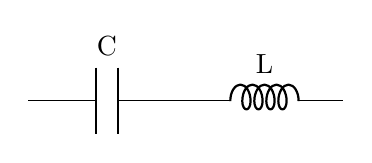
\begin{tikzpicture}
\draw (0,0) to[C, label=C] ++(2,0)
to[L, label=L] ++(2,0);
\end{tikzpicture}
\end{center}

Things become even more stark when a resistor is added in series:

\begin{center}
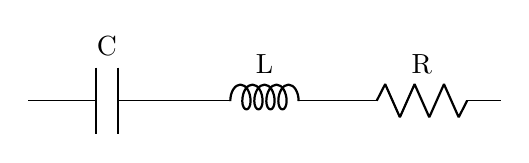
\begin{tikzpicture}
\draw (0,0) to[C, label=C] ++(2,0)
to[L, label=L] ++(2,0)
to[R, label=R] ++(2,0);
\end{tikzpicture}
\end{center}

In order to truly achieve the results seen in our data, we would likely need to add a resistor in parallel with the capacitor. We may even need to add leading and trailing resistance and inductance. However, modeling this will be left as an exercise to the reader.

\subsection{Inductor}

An ideal inductor has no self-resonsnt frequency or peak in the S-Parameter curve:

        \begin{center}
        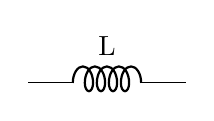
\begin{tikzpicture}
            \draw (0,0) to[L, label=L] ++(2,0);
        \end{tikzpicture}
        \end{center}

However, when you add a capacitor in parallel, the peak appears:

        \begin{center}
        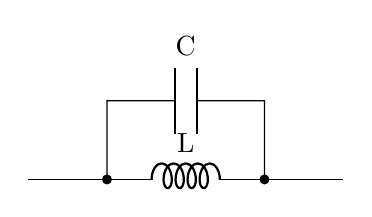
\begin{tikzpicture}
            \draw (0,0) to[L, label=L] ++(4,0);
            \draw (1, 0) to[short, *-] ++(0, 1)
            to[C, label=C] ++(2, 0)
            to[short, -*] ++(0, -1);
        \end{tikzpicture}
        \end{center}

Things again become stark when an inductor is added in series:

        \begin{center}
        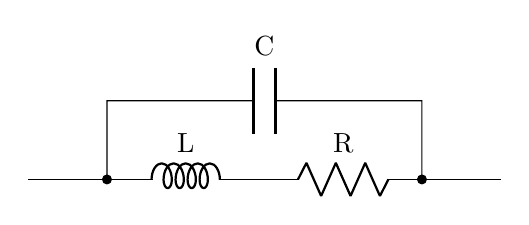
\begin{tikzpicture}
            \draw (0,0) to[short] ++(1,0)
            to[L, label=L] ++(2,0)
            to[R, label=R] ++(2,0)
            to[short] ++(1, 0);
            \draw (1, 0) to[short, *-] ++(0, 1)
            to[C, label=C] ++(4, 0)
            to[short, -*] ++(0, -1);
        \end{tikzpicture}
        \end{center}

On additional corection to best fit the data would be to add a resistor in parallel with the inductor. However, modeling this will again be left as an exercise to the reader.

\section{Conclusion}

Modeling real-world passive components can be an important exercise in circuit design. We have seen in this lab that these components do not act in accordance with their theoretical models. This is especially true at higher frequencies.

Rather, capacitors and inductors seem to have a {\it{self-resonant frequency}} at which the S-Parameters either dip or peak. If frequency is increased beyond this point, each component appears to act like the other.

If a RF circuit is to be built using these higher frequencies, maintaining the parasitic component models in mind (and measuring them if necessary) should be an important consideration.


\section*{Acknowledgments}
Special thanks to my lab partners Devorah and Marc for all their help and support. They have lent several of their figures to match the data which I collected in my lab notebook. Thanks also to Yifan for inspiring me to dust off my \LaTeX skills, as well as helping with several of the Tikz schematics. Finally, thanks to Joanna and Steve for their endless patience in my quest to learn electronics.

%{\appendices
%\section*{Proof of the First Zonklar Equation}
%Appendix one text goes here.
% You can choose not to have a title for an appendix if you want by leaving the argument blank
%\section*{Proof of the Second Zonklar Equation}
%Appendix two text goes here.}


% \begin{thebibliography}{1}
% \bibliographystyle{IEEEtran}

% \bibitem{ref1}
% {\it{Mathematics Into Type}}. American Mathematical Society. [Online]. Available: https://www.ams.org/arc/styleguide/mit-2.pdf

% \end{thebibliography}

\end{document}


